% Better horizontal rules
\usepackage{booktabs}

% Use Tikz (and other pkgs) for Ben's picture
% xcolor MUST come first!!! https://en.wikibooks.org/wiki/LaTeX/Colors
\usepackage[usenames,dvipsnames]{xcolor}
\usepackage{tikz}
\usepackage{graphicx}
\usepackage{multicol}

% Override Scribble's default SecRef to numeric only
\renewcommand{\SecRef}[2]{~#1}

\hypersetup{hidelinks} 

\usepackage[scaled=0.95]{zi4}
\usepackage[T1]{fontenc}

% For bib style
\newcommand{\Thyperref}[2]{\hyperref[#2]{#1}}

% Disable hrule for figures
\renewcommand{\Legend}[1]{~ \vspace{4pt} \legend{#1}}

%%% From Ben's treepict work

%% Import and print the pictures for a project
%% Arguments:
%% - Name of the project
\newcommand{\pict}[1]{\begin{tabular}{c}\scalebox{0.6}{\input{module-graphs/#1}}\end{tabular}}

\newcommand{\rkt}[2]{$\bullet$}

%% To show overfull, turn off for production!!!
\overfullrule=1mm

%% Artifact badge!
\usepackage[firstpage]{draftwatermark}
\SetWatermarkText{\hspace*{8in}\raisebox{7.0in}{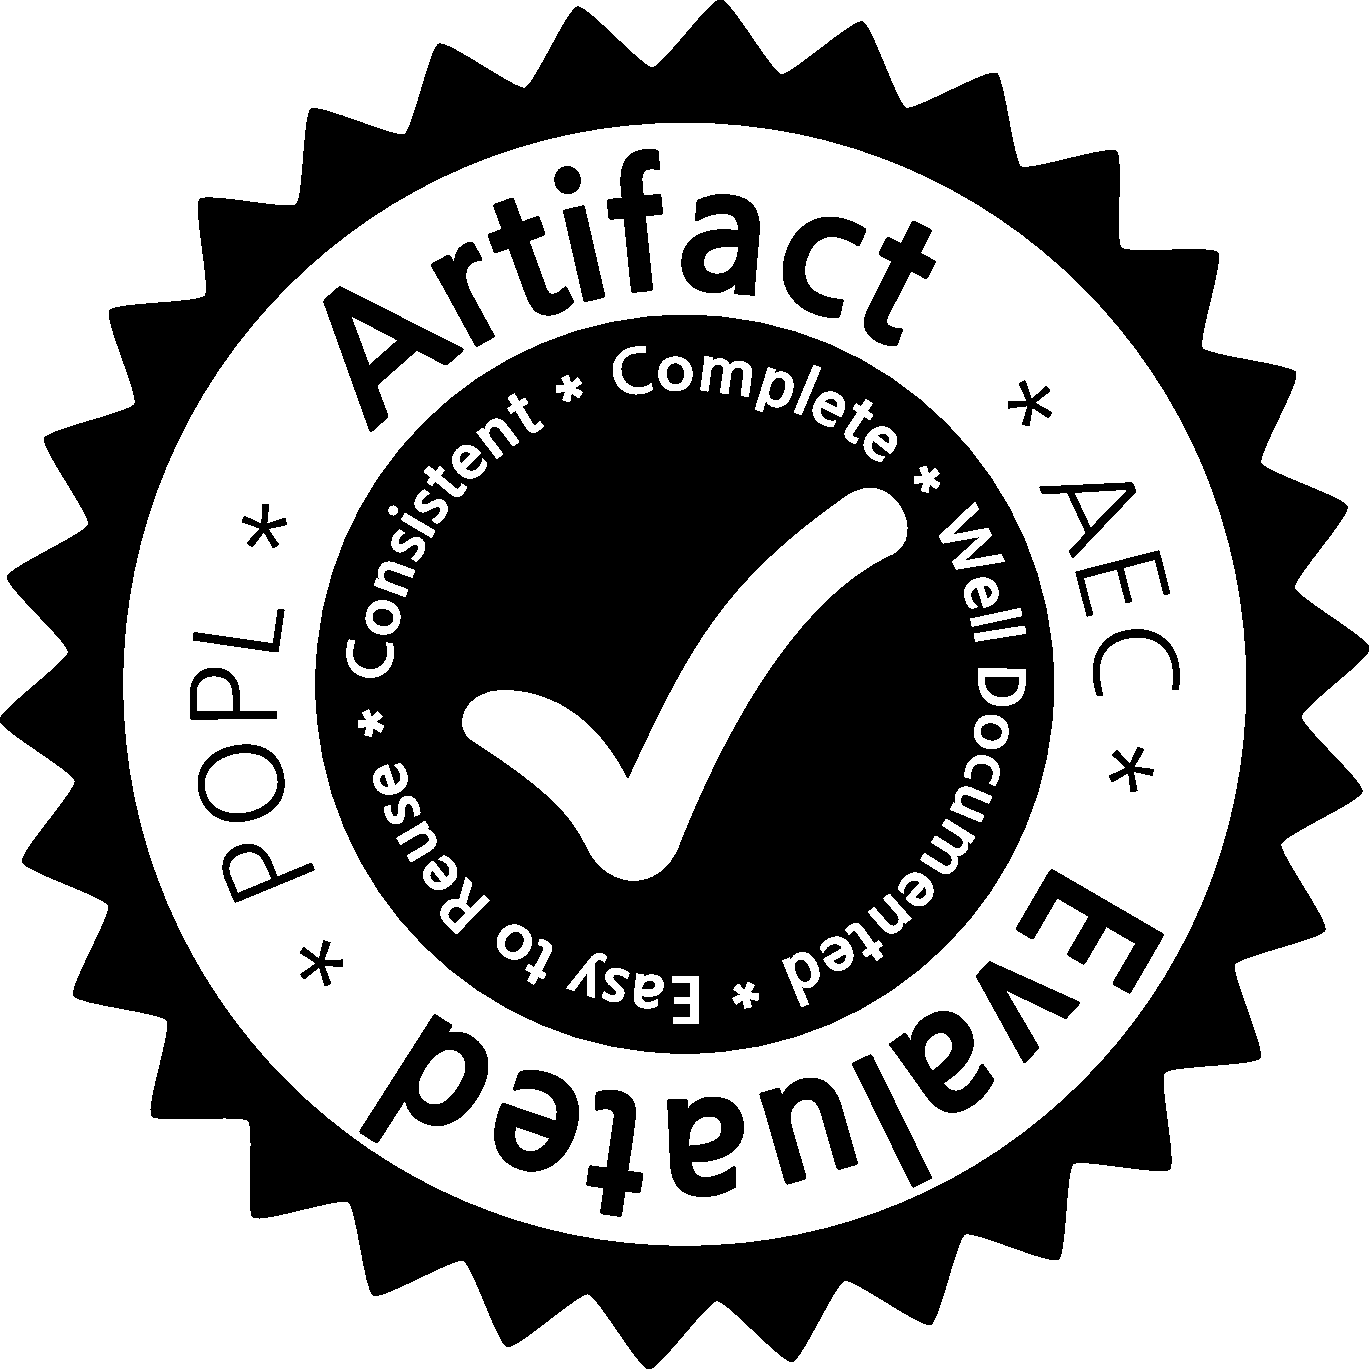
\includegraphics[scale=0.1]{aec-badge-popl}}}
\SetWatermarkAngle{0}

%% balance last page columns
\usepackage{flushend}

%% for figure 2
\let\ulcorner\relax
\let\urcorner\relax
\let\llcorner\relax
\let\lrcorner\relax
\usepackage{amssymb}
\let\Asterisk\relax
\let\Square\relax
\usepackage{bbding}
